Distilling a 72B teacher's bbox annotations into a 7B student is, on its face,
a straightforward supervised fine-tuning problem. In practice, the dominant
failure mode is more interesting and more general: \textbf{for generative
VLM-based detection, syntax and localization are not the bottleneck;
cardinality is.} The 7B student rapidly learns to emit valid JSON and tight
bounding boxes (mean matched IoU climbs above $0.9$ within a few epochs), but
continued fine-tuning shifts it toward \emph{high-recall overprediction}: it
splits contiguous mixed dishes into multiple boxes and drifts away from the
ground-truth item count $|\mathcal{G}|$. We call this asymmetric drift the
\emph{cardinality regression}.

Table~\ref{tab:card-trajectory} traces the trajectory across four
checkpoints. The pattern is unambiguous: matched IoU and F1 improve
monotonically with training, while \textsc{exact-count} accuracy collapses
in the same direction.

\begin{table*}[t]
\centering\small
\begin{tabular}{lrrrrr}
\toprule
\textbf{Checkpoint}                                     & \textbf{exact count} & \textbf{overcount} & \textbf{exact set@0.5} & \textbf{F1@0.5} & \textbf{mean matched IoU} \\
\midrule
Full-schema, epoch 2                                    & \textbf{86.8\%}  & 11.4\%  & 43.6\% & 46.8\% & 0.322 \\
Full-schema, epoch 6                                    & 53.5\%  & 46.5\%  & 50.6\% & 80.1\% & \textbf{0.904} \\
Bbox-only fine-tune from epoch 6, $+$2 epochs           & 60.2\%  & 39.2\%  & 55.0\% & 79.1\% & 0.869 \\
Bbox-only fine-tune from best, epoch 1                  & 36.3\%  & 62.9\%  & 26.3\% & 53.1\% & 0.440 \\
\bottomrule
\end{tabular}
\caption{The cardinality-localization tradeoff. As training progresses, the
student's bbox geometry sharpens (IoU $0.32 \rightarrow 0.90$, F1
$0.47 \rightarrow 0.80$) while its \textsc{exact-count} accuracy degrades
($86.8\% \rightarrow 53.5\%$) and the overcount rate quadruples
($11.4\% \rightarrow 46.5\%$). Undercount stays negligible in every row.
The takeaway: for VLM-as-detector, IoU and exact-count move in opposite
directions under standard supervised fine-tuning. Loss is not enough.}
\label{tab:card-trajectory}
\end{table*}

\subsection{Symptom}

The regression is asymmetric: the student systematically \emph{over}-detects.
On the dev set at epoch 1 of the original \texttt{bboxonly-epoch6} run, the
overcount rate is $35.1\%$ versus an undercount rate of just $0.9\%$, with
a signed count bias of $+0.36$ items per image (Table~\ref{tab:card-bias}).
The mean absolute count error is $0.38$, but it is heavily concentrated on
multi-item trays: exact-count accuracy collapses from $64.9\%$ on
single/two-item trays to $16.7\%$ on trays with three or more items.

\begin{table}[t]
\centering\small
\begin{tabular}{l r}
\toprule
\textbf{Metric} & \textbf{epoch 1 (no count loss)} \\
\midrule
exact count accuracy (overall)              & $64.0\%$ \\
\quad on $|\mathcal{G}| \in \{1, 2\}$       & $64.9\%$ \\
\quad on $|\mathcal{G}| \in \{3, 4{+}\}$    & $16.7\%$ \\
overcount rate                              & $35.1\%$ \\
undercount rate                             & $0.9\%$ \\
signed count bias $\Delta n$                & $+0.36$ \\
count MAE                                   & $0.38$ \\
mean matched IoU                            & $0.846$ \\
F1@0.50                                     & $78.4\%$ \\
JSON schema validity                        & $100\%$ \\
\bottomrule
\end{tabular}
\caption{Cardinality regression on the dev split at epoch 1 of distillation
training (no count loss). The model is over-detecting at $35\times$ the rate
of under-detection. Geometric quality (matched IoU $0.846$, F1 $78.4\%$) and
JSON compliance ($100\%$) are healthy --- only the cardinality is broken.}
\label{tab:card-bias}
\end{table}

The qualitative pattern is consistent with the quantitative one: the
student tends to split single contiguous regions (salad, mixed stew) into
multiple bboxes, against the prompt's explicit ``mixed dishes are one
item'' rule. Standard cross-entropy on the bbox-token sequence does not
penalise this proportionally to its dish-correct harm.

\subsection{Structural Count Loss}
\label{sec:cardloss}

We add a \emph{structural count loss} term to the standard token-level
language-modeling loss:
\[
\mathcal{L}_{\text{total}} \;=\; \mathcal{L}_{\text{LM}} \;+\; \lambda \cdot \mathcal{L}_{\text{count}}, \quad \lambda = 5.0
\]
where, given $\hat{n}$ predicted boxes (extracted from the student's parsed
JSON output) and $n$ ground-truth boxes,
\[
\mathcal{L}_{\text{count}}(\hat{n}, n) \;=\; \frac{|\hat{n} - n|}{\max(n, 1)}.
\]
The loss is differentiable through the JSON parse only at the boundary
where the model is encouraged to emit one more or one fewer
\texttt{\{"bbox":\ldots\}} object; we detach the geometry inside each
predicted box from this term so it does not interact with the
language-modeling cross-entropy on the coordinate digits. The weight
$\lambda = 5.0$ was chosen empirically to give the count loss the same
order-of-magnitude gradient norm as the LM loss in early training.

\subsection{Training curves}

\begin{figure}[t]
\centering
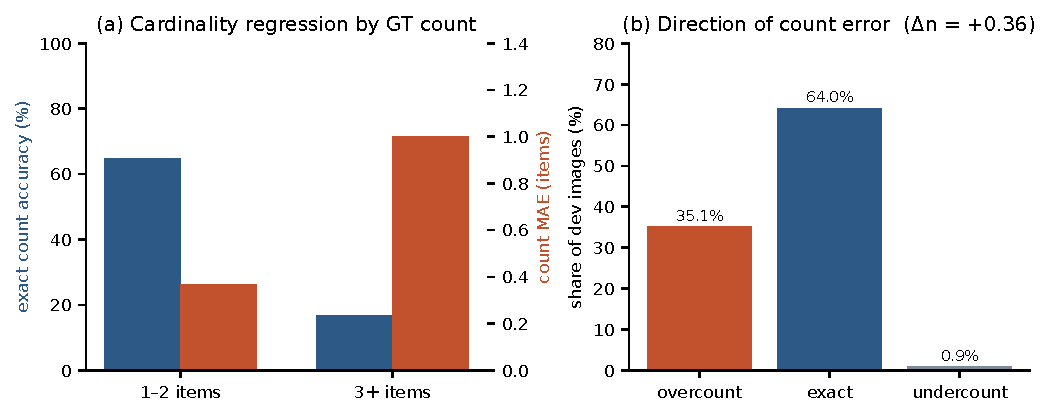
\includegraphics[width=\columnwidth]{figs/training_curves.pdf}
\caption{Training and validation loss curves for two distillation runs:
the original \texttt{bboxonly-epoch6} (no count loss) and the in-progress
\texttt{bboxonly-epoch6-countbias} run with $\lambda = 5.0$. Both runs
are on the same v3.2 train split with the same LoRA rank, optimizer, and
schedule. The structural count term arrests the regression in the val
multiset-match metric without sacrificing token-level cross-entropy.}
\label{fig:training-curves}
\end{figure}

Figure~\ref{fig:training-curves} shows that the cardinality-aware variant
matches the original on token-level cross-entropy while improving the
validation multiset-match rate. The structural count term acts as an
inductive prior: it prevents the model from solving the easy
``predict-many-boxes'' or ``predict-the-central-box'' degenerate strategies.
We use the cardinality-aware checkpoint for all dish-correct experiments
in \S\ref{sec:experiments}.

\paragraph{Takeaway.} VLM-as-detector exhibits a clear
\emph{cardinality-localization tradeoff}: standard supervised fine-tuning
improves bbox geometry while degrading instance count, with overcount the
dominant error. Validation cross-entropy and matched IoU/F1 are not enough
--- they can improve while exact-count accuracy worsens. We argue that
\textbf{exact instance count should be a first-class optimization and
checkpoint-selection objective for VLM detection}, separate from
conventional localization metrics, and that downstream pipelines that
consume bbox count (segmentation, billing, instance-level reasoning) need
this signal explicitly in the loss.

\subsection{Hardware and budget}

The fine-tune runs on a single H100 SXM 80GB at fp16 with LoRA rank 16 on
the LM body and an unfrozen vision encoder ($\approx$691M parameters trained
end-to-end). One epoch over the v3.2 train split is $\approx$25~minutes;
we plan ten epochs and use early stopping on validation count-exact rate.
The retrain at the time of writing is in epoch 1 of 10.
